\documentclass[12pt,letterpaper]{ctexart}
\usepackage{fullpage}
\usepackage[top=2cm, bottom=4.5cm, left=2.5cm, right=2.5cm]{geometry}
\usepackage{amsmath,amsthm,amsfonts,amssymb,amscd}
\usepackage{lastpage}
\usepackage{enumerate}
\usepackage[binary-units=true]{siunitx}
\usepackage{fancyhdr}
\usepackage{mathrsfs}
\usepackage{xcolor}
\usepackage{graphicx} %插入图片的宏包
\usepackage{float} %设置图片浮动位置的宏包
\usepackage{subfigure} %插入多图时用子图显示的宏包
\usepackage{listings}
\usepackage{afterpage}
\usepackage{hyperref}
\hypersetup{
    colorlinks=true,
    linkcolor=blue,
    filecolor=magenta,
    urlcolor=cyan,
}

\newcommand\blankpage{%
  \null
  \thispagestyle{empty}%
  \addtocounter{page}{-1}%
  \newpage
}


\hypersetup{%
  colorlinks=true,
  linkcolor=blue,
  linkbordercolor={0 0 1}
}

\renewcommand\lstlistingname{Algorithm}
\renewcommand\lstlistlistingname{Algorithms}
\def\lstlistingautorefname{Alg.}

\lstdefinestyle{Python}{
    language        = Python,
    frame           = lines,
    basicstyle      = \footnotesize,
    keywordstyle    = \color{blue},
    stringstyle     = \color{green},
    commentstyle    = \color{red}\ttfamily
}

\setlength{\parindent}{0.0in}
\setlength{\parskip}{0.05in}

% Edit these as appropriate
\newcommand\course{CS305}
\newcommand\hwnumber{1}                  % <-- homework number
\newcommand\NetIDa{11711918}           % <-- NetID of person #1
\newcommand\NetIDb{吴烨昌}           % <-- NetID of person #2 (Comment this line out for problem sets)

\pagestyle{fancyplain}
\headheight 35pt
\lhead{\NetIDa}
\lhead{\NetIDa\\\NetIDb}                 % <-- Comment this line out for problem sets (make sure you are person #1)
\chead{\textbf{\Large Homework \hwnumber}}
\rhead{\course \\ \today}
\lfoot{}
\cfoot{}
\rfoot{\small\thepage}
\headsep 1.5em

\begin{document}

\section*{Problem 1}

{\bf Description}

Compare packet switch and circuit switch under the following scenario.
Suppose you would like to deliver a message of $x$ bit.
There are $k$ links from the source to destination.
The propagation delay of each link is $d$ second, the transmission rate is $b$ bit/second.
The circuit setup time under circuit switch is $s$ second.
Under packet switch network, when the packet length is $p$ bit, the queue delay in every node can be neglected.
Please calculate the condition, under which the delay of packet switch is smaller than that of the circuit switch.

{\bf Solution}

  In circuit switch, total delay is

  $$
  t_{c} = s + k \times d + \frac{x}{b}
  $$

  In packet switch, total delay is

  $$
  t_{s} = \frac{(k - 1) \times p }{b} + \frac{x}{p} \times \frac{p}{b} + k \times  d
  $$

  When $t_s < t_c$, or $ (k - 1) p < sb$, the delay of packet switch is smaller than that of the circuit switch.

\newpage

\section*{Problem 2}

{\bf Description}

Calculate the overall delay of transmitting a \SI{1000}{\kilo\byte} file under the following circumstance.
The overall delay is defined as the time from the starting point of the transmission until the arrival of the last bit to the destination.
RTT is assumed to be \SI{100}{\ms}, one packet is \SI{1}{\kilo\byte} (\SI{1024}{\byte}) size.
The handshaking process costs \SI{2}{RTT} before transmitting the file.
% Rest of the work...
\begin{enumerate}
  \item Transmission bandwidth is \SI[per-mode=symbol]{1.5}{\mega\bit\per\second}, the packets can be continuously transmitted.
  \item Transmission bandwidth is \SI[per-mode=symbol]{1.5}{\mega\bit\per\second}, but when one packet is transmitted, the next packet should wait for 1 RTT (waiting for the acknowledgement of the receiver) before being transmitted.
  \item Transmission bandwidth is infinite, i.e. transmission delay is 0. After every \SI{1}{RTT}, as many as 20 packets can be transmitted.
\end{enumerate}

{\bf Solution}

The number of packets $n$ is $\frac{1000\text{kB}}{1\text{kB}}=1000$.

\begin{enumerate}
  \item The delay under {\bf circumstance 1}

  $$
  t_1 = 2\text{RTT} + n \times \frac{1\text{KB} \times 8\text{b/B}}{1.5\text{Mb/s}} + 0.5\text{RTT} \approx 5.711\text{s}
  $$

  \item The delay under {\bf circumstance 2}

  $$
  t_2 = 2\text{RTT} + n \times (\frac{1\text{KB}\times 8\text{b/B}}{1.5\text{Mb/s}} + \text{RTT}) - \text{RTT} = t_1 + (n - 1) \text{RTT} \approx 105.611\text{s}
  $$

  \item The delay under {\bf circumstance 3}

  $$
  t_3 = 2\text{RTT} + \frac{n}{20/\text{RTT}} = 52\text{RTT} = 5.2\text{s}
  $$
\end{enumerate}

\section*{Problem 3}

{\bf Description}

List six access technologies. Classify each of them as home access, enterprise access, or wide-area mobile access.

{\bf Solution}

\begin{itemize}
  \item Home access: Dial-up modem over telephone line, Hybrid fiber-coaxial cable, WLAN
  \item Enterprise access: IEEE 802.1X
  \item Wide-area mobile access: 3G, 4G, 5G
\end{itemize}

\section*{Problem 4}
{\bf Description}

\begin{enumerate}
  \item List five nonproprietary Internet applications and the application-layer protocols that they use.
  \item What information is used by a process running on one host to identify a process running on another host?
\end{enumerate}

{\bf Solution}

\begin{enumerate}
  \item As followed
  \begin{enumerate}
    \item  web: http/https
    \item e-mail: imap/smtp/pop3
    \item remote desktop: rdp
    \item file transform: ftp
    \item remote access: ssh, telnet
  \end{enumerate}
  \item The IP address and port number of the destination host
\end{enumerate}

\newpage

\chead{\textbf{\Large Lab 3}}
\section*{Problem 1}

{\bf Description}

Using cURL to make request, attach the screenshot of curl result and packets captured by Wireshark. And answer

\begin{enumerate}
  \item What did you get via cURL?
  \item What are the meaning of fields in your request and response headers?
  \item Is the packet captured by Wireshark capture correspond to the cURL request?
\end{enumerate}

for following request:
\begin{enumerate}
  \item GET request to \url{http://httpbin.org/get}
  \item POST request to \url{http://httpbin.org/post}
\end{enumerate}

{\bf Solution}

\begin{enumerate}
  \item GET request to \url{http://httpbin.org/get}
    \begin{enumerate}
      \item Screenshot of cURL result(Figure~\ref{fig:get_cmd})
        \begin{figure}[H]
          \centering
          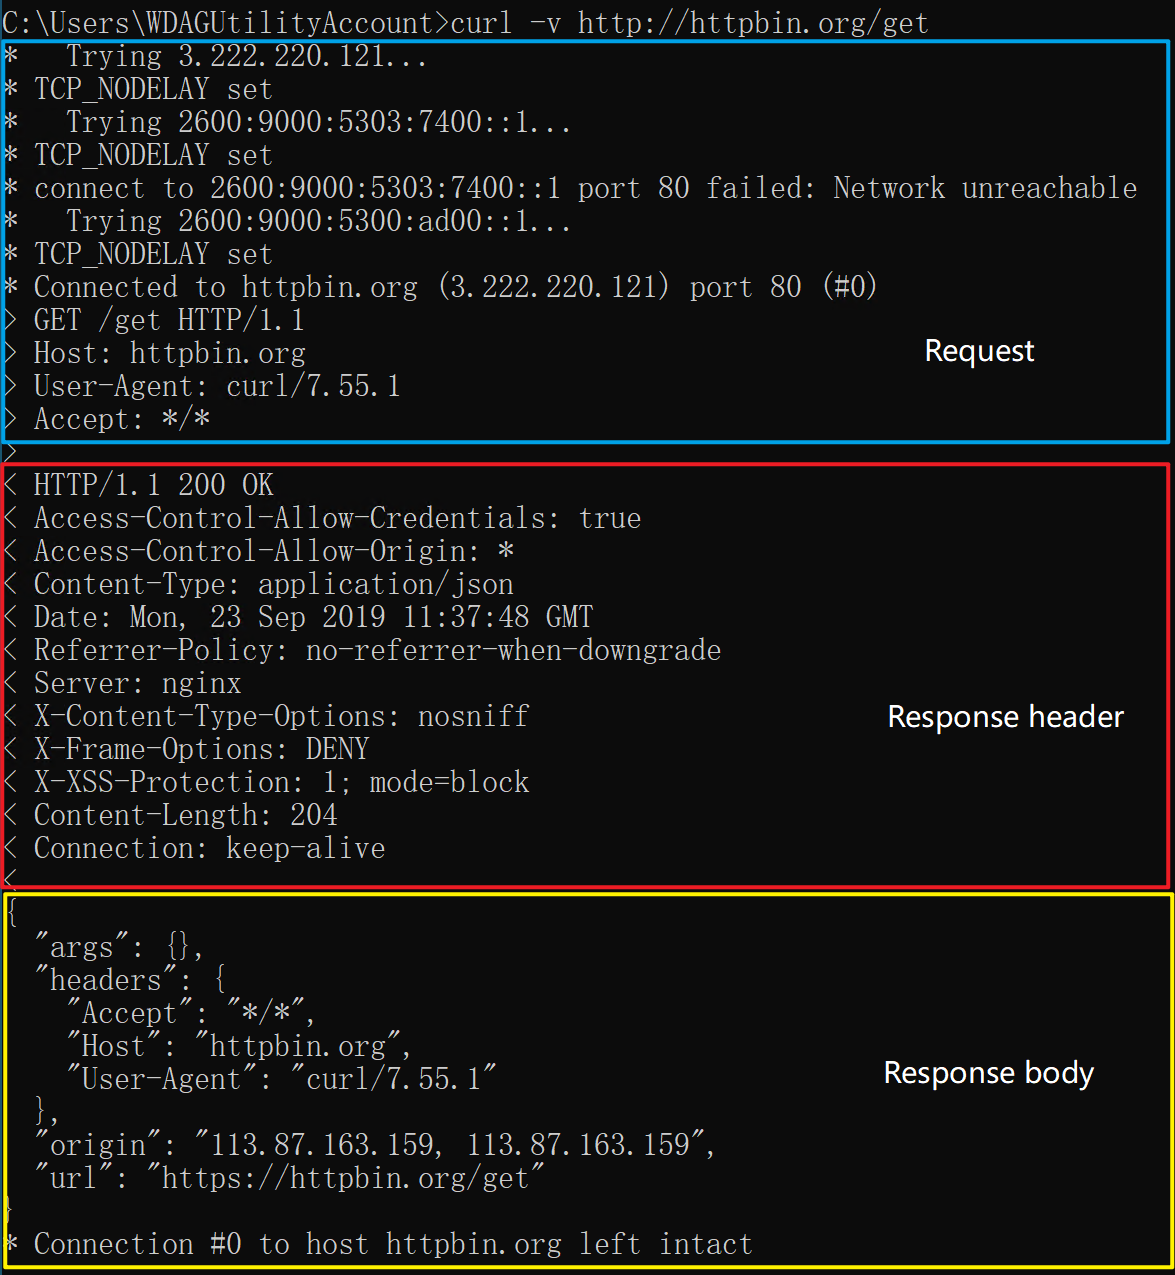
\includegraphics[width=0.8\linewidth]{assets/get_cmd.png}
          \caption{cURL output when making GET request}
          \label{fig:get_cmd}
        \end{figure}
      \item Screenshot of packets captured by Wireshark(Figure~\ref{fig:get_ws})
        \begin{figure}[H]
          \centering
          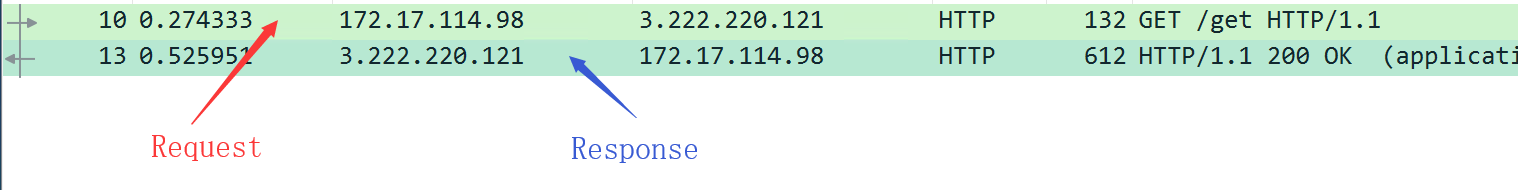
\includegraphics[width=0.8\linewidth]{assets/get_wireshark.png}
          \caption{Traffic captured by WireShark while making GET request}
          \label{fig:get_ws}
        \end{figure}
      \newpage
      \item Request
        \begin{itemize}
          \item request type: GET
          \item protocol: HTTP/1.1
          \item host: httpbin.org
          \item user-agent: curl/7.55.1
        \end{itemize}
      \item Response
        \begin{itemize}
          \item status code: 200 (OK)
          \item content type: application/json
          \item server: nginx
          \item content-length: 204
          \item Others: Access-Control-Allow-Origin: * (允许跨域)
        \end{itemize}

    \end{enumerate}
  \newpage
  \item POST request to \url{http://httpbin.org/post}
  \begin{enumerate}
    \item Screenshot of cURL result(Figure~\ref{fig:post_cmd})
      \begin{figure}[H]
        \centering
        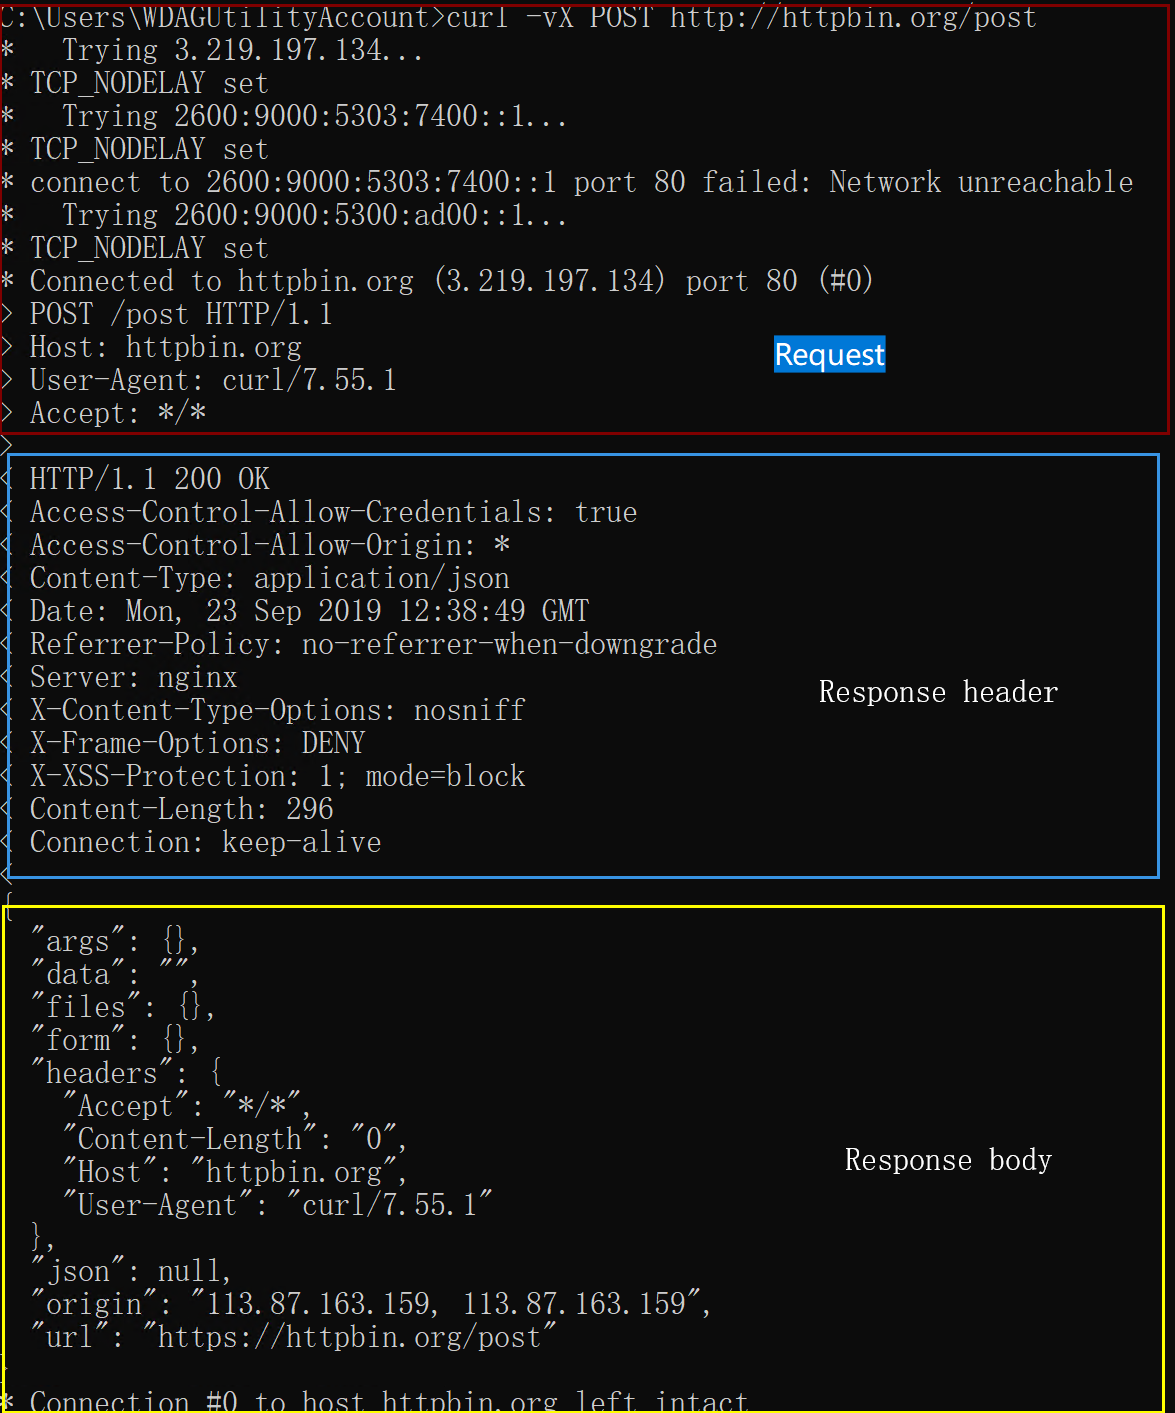
\includegraphics[width=0.8\linewidth]{assets/post_cmd.png}
        \caption{cURL output when making GET request}
        \label{fig:post_cmd}
      \end{figure}
    \newpage
    \item Screenshot of packets captured by Wireshark(Figure~\ref{fig:post_ws})
      \begin{figure}[H]
        \centering
        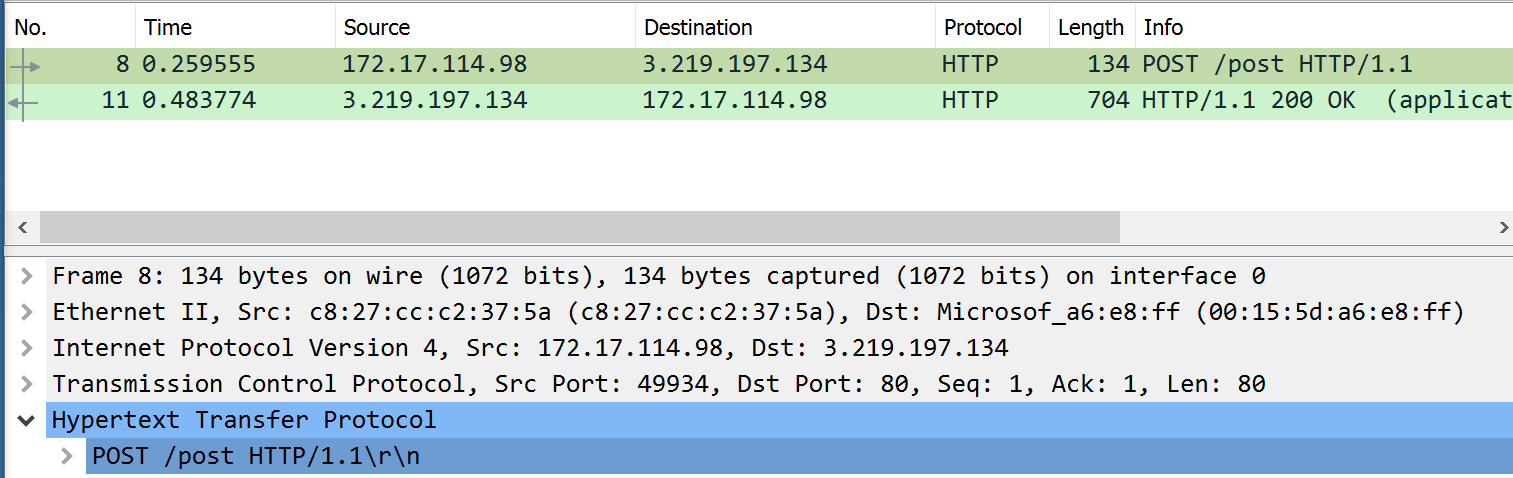
\includegraphics[width=0.8\linewidth]{assets/post_wireshark.png}
        \caption{Traffic captured by WireShark while making GET request}
        \label{fig:post_ws}
      \end{figure}
    \item Request
      \begin{itemize}
        \item request type: POST
        \item protocol: HTTP/1.1
        \item host: httpbin.org
        \item user-agent: curl/7.55.1
      \end{itemize}
    \item Response
      \begin{itemize}
        \item status code: 200 (OK)
        \item content type: application/json
        \item server: nginx
        \item content-length: 296
        \item Others: Access-Control-Allow-Origin: * (允许跨域)
      \end{itemize}

  \end{enumerate}
\end{enumerate}

\end{document}
